
% !TeX root = ../book.tex
% !TeX spellcheck = fr_FR
% !TeX encoding = ISO-8859-1

\section{Petit r�tro avec long d�placement}\label{sec:B10}

Ce point est assez difficile. Il demande une grande souplesse et une
bonne ma�trise du r�tro. Il conviendra de bien s'entra�ner sur cette
figure afin de gagner en confiance et de sentir d�j� les trois billes
dans le coin avant de jouer.

Comme le montre la figure, notre position au � milieu du jeu de quilles
� est tr�s inconfortable. Seule la bille 3 occupe une position
favorable. N'allons pas trop vite. Examinons bien avant de prendre notre
d�cision. Remarquons que la direction 1-2 coupe le haut de la table aux
environs du coin diam�tralement oppos� � la 3, disons dans le carr� du
coin : nous sommes sauv�. Appliquons un r�tro direct, petite fl�che,
main arri�re loin sur la canne, coup tr�s souple et pas trop fort, effet
� droite avec tenue l�g�re. Si la 2 touche la petite bande du haut,
l'effet favorisera sa rentr�e, si elle touche la grande, l'effet
retiendra son �cartement. Dans les deux cas, la 2 rentrera dans le coin
de la 3.

Deuxi�me solution : un 1B via la grande bande � notre gauche (en
pointill� sur la figure) est possible. Il s'agit d'un angle de 80�
environ, petite fl�che, main arri�re loin sur la canne, effet � gauche
bas de bille, coup souple et pas trop fort. Cette solution est plus
rassurante mais plus difficile. Elle demande une grande souplesse et la
grosseur de la prise sera fonction de la direction � donner � la 2 afin
qu'elle rentre au coin de la 3.

Remarques :

\begin{itemize}
	\item si la position est favorable, donnez la pr�f�rence au r�tro. C'est le
		meilleur moyen de ma�triser les billes .... � condition de bien
		ma�triser le r�tro !
	\item si la direction 1-2 coupe la petite bande oppos�e un peu loin du coin, 30, 40 cm, tentez le 1B souple.
	\item si la direction 1-2 coupe la petite bande ou la grande trop loin du
		coin, choisissez une autre solution car le rappel deviendrait vite
		impossible
\end{itemize}


\begin{figure}[htb]
	\centering
	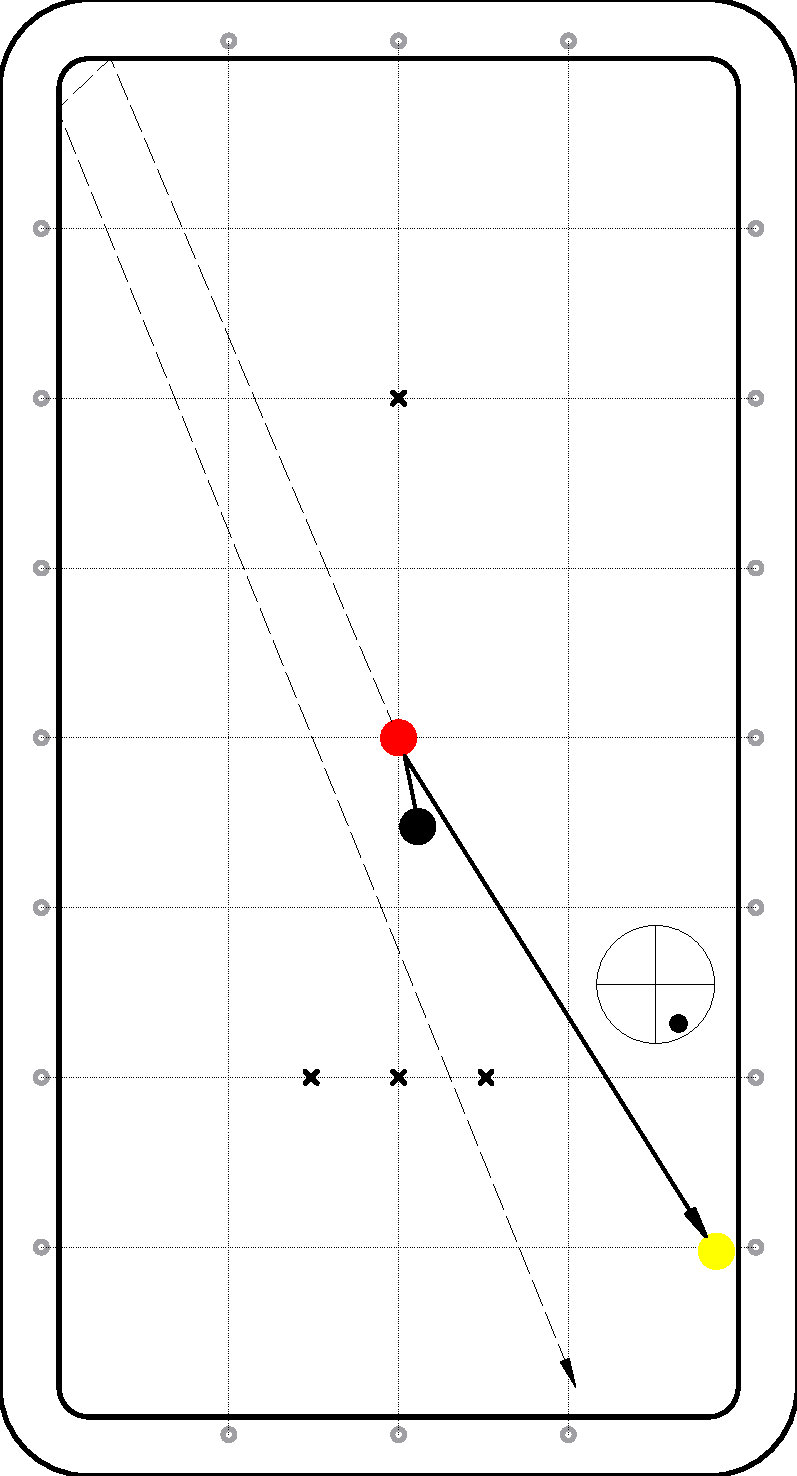
\includegraphics[width=0.85\linewidth]{B/imagesB/B10-01.pdf}
	\caption{Petit r�tro avec long d�placement}
	\label{fig:B10-1}
\end{figure}

\clearpage
